\section{Development view}
De development view is gefocust op het in beeld brengen van de organisatie van software modules \parencite{4p1Model}.
Om dit in beeld te brengen is er gebruikgemaakt van een component diagram.

\whitespace
In figuur \ref{fig:ComponentDiagram} is een component diagram gemaakt.
In het diagram is te zien dat er gebruikgemaakt wordt van een externe authenticatie provider.
Verder is de SOLID implementatie terug te vinden in het diagram (zie \ref{subsecion:SoftwareArhitectuur} voor meer informatie). 
% \todo[inline]{Ik ben het meest onzeker over dit diagram. Want ik heb een gevoel dat ik het veel te erg gegeneraliseerd heb.}

\whitespace[2]
\begin{graphic}
    \captionsetup{type=figure}
    \caption{Deployment diagram van het afstudeerproduct}
    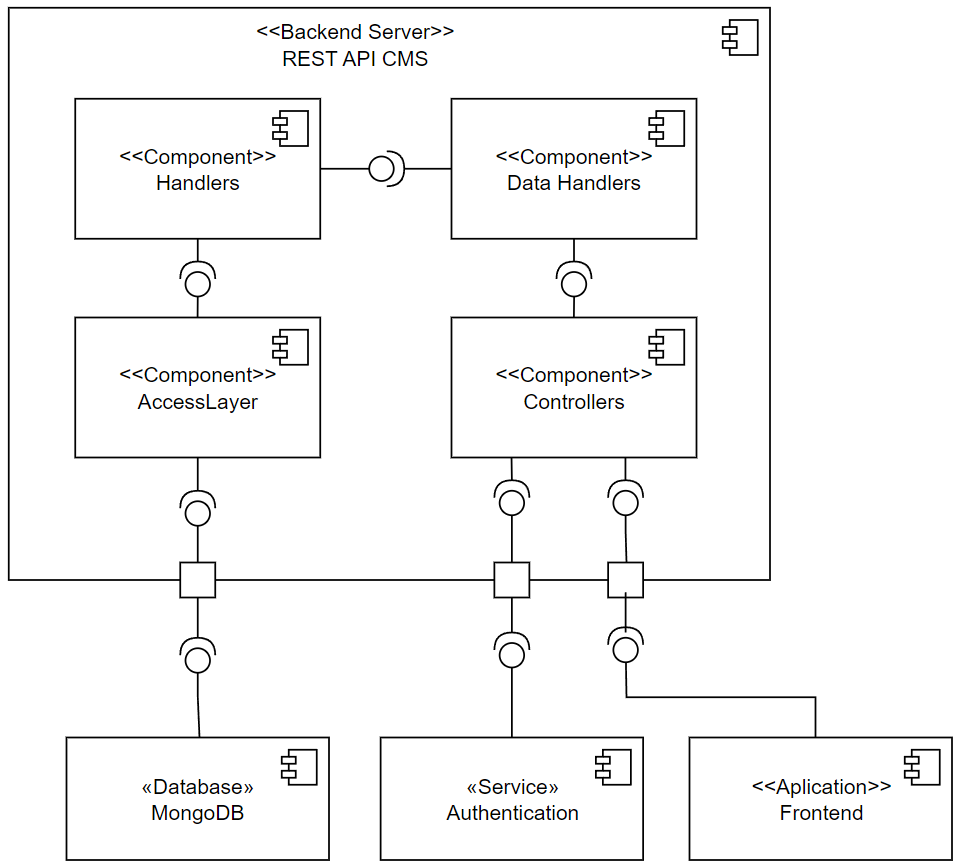
\includegraphics[scale=0.32]{ComponentDiagram.png}
    \label{fig:ComponentDiagram}
\end{graphic}
